% !TeX spellcheck = en_GB

\documentclass[]{beamer}

\usepackage[utf8]{inputenc}
\usepackage[english]{babel}
\usepackage{tabularx}
\usepackage[backend=bibtex]{biblatex}
\usepackage[percent]{overpic}
\usepackage{mathtools}
\usepackage{listings}

\usepackage{tikz}
\usetikzlibrary{chains,shapes.multipart}
\usetikzlibrary{shapes,calc,positioning}


\tikzset{
	queue/.pic={
		\draw[line width=1pt]
		(0,0) -- ++(.75cm,0) -- ++(0,-1cm) -- ++(-.75cm,0);
		\foreach \Val in {1,...,#1}
		\draw ([xshift=-\Val*10pt].75cm,0) -- ++(0,-1cm); 
	},
}

\usetheme{metropolis}

\bibliography{biblio.bib}

\title{Computer Systems}
\subtitle{Exercises on Fundamental Laws - Lazowska chap.3}

\author{Stefano Cereda \\ stefano.cereda@polimi.it \\
\includegraphics[width=0.1\linewidth]{../you}}
\date{06/05/2019}
\institute[PoliMi]{\centering Politecnico di Milano \\ \vspace{0.2cm}
	\includegraphics[width=0.2\linewidth]{../logopolimi}}
%\logo{\includegraphics[width=10mm]{../logopolimi}}

\setbeamercovered{invisible}

\makeindex

\begin{document}

\begin{frame}
	\maketitle
\end{frame}

%\begin{frame}
%Everybody is moving to cloud:
%\includegraphics[width=\linewidth]{images/cloud_tweets.png}
%\cite{roundup-of-cloud-computing-forecasts}
%
%Amazon offers 84 different instance types on AWS, which ones and how many do you select? 
%\end{frame}

\begin{frame}{Recap - Basic Quantities}
\centering
\begin{tabular}{ccc}
    \emph{$T$}	&	length of an observation interval  &   \\
    \emph{$A_k$}	&	number of arrivals observed    &   \\
    \emph{$C_k$}	&	number of completions observed &   \\
    \emph{$\lambda_k$}	&	arrival rate &   $\lambda_k \equiv 	\frac{A_k}{T}$  \\
    \emph{$X_k$}	&	throughput    &   $X_k \equiv \frac{C_k}{T}$  \\
    \emph{$B_k$}	&	busy time  &   \\
    \emph{$U_k$}	&	utilization    &   $U_k \equiv \frac{B_k}{T}$  \\
    \emph{$S_k$}	&	service requirement per visit	&	$S_k \equiv \frac{B_k}{C_k} = \frac{U_k T}{C_k}$    \\
    \emph{$W$}      &   accumulated system time   &   \\
    \emph{$N$}      &	customer population  &   $N \equiv \frac{W}{T}$    \\
    \emph{$R_k$}	&	residence time   &   $R_k \equiv \frac{W}{C_k}$    \\
    \emph{$Z$}      &	think time of a terminal user &  \\
    \emph{$V_k$}	&	number of visits &   $V_k \equiv \frac{C_k}{C}$   \\
    \emph{$D_k$}	&	service demand   &   $D_k \equiv V_k S_k = \frac{B_k}{C} = \frac{U_k T}{C}$    \\
\end{tabular}
\end{frame}

\begin{frame}{Recap - Fundamental Laws}
\centering
\begin{tabular}{cc}
	Utilization Law:	&	$U_k = X_k S_K = X D_k$ \\
	Little's Law:		&	$N = X R$	\\
	Response Time Law:	&	$R = \frac{N}{X} - Z$	\\
	Forced Flow Law:	&	$X_k = V_k X$	\\
\end{tabular}
\end{frame}

\begin{frame}[allowframebreaks]{Example on Little's Law \cite{little2008little}}
Caroline is a wine buff and bon vivant. She likes to stop at her local wine store, \emph{Transcendental Tastings}, on the way home from work. She browses the aisles looking for the latest releases from her favorite vineyards. Occasionally she picks up a few bottles. She stores these in a rack in a cool corner of her cellar. She and her partner eat out frequently but when they are at home they usually split a bottle of wine at dinner. Sometimes they have friends over and that puts a bigger dent in the wine inventory.

They have been doing this for some time. Her wine rack holds 240 bottles. She notices that she seldom fills the rack to the top but sometimes after a good party the rack is empty. On average it seems to be about 2/3rds full, which would equate to 160 bottles.

Many wines improve with age. After reading an article about this, Caroline starts to wonder how long, on average, she has been keeping her wines. She went back through a few months of wine invoices from \emph{Transcendental} and estimates that she has bought, on average, about eight bottles per month. But she certainly doesn't know when she drank which bottle and so there seems to be no way she can find out, even approximately, the average age of the bottles she has been drinking.

This is a good task for Little's Law.
\end{frame}

\begin{frame}
\centering
\begin{overpic}[width=0.5\textwidth]{images/wine_rack}
\put (-30,50) {$\xRightarrow{\text{96 bot/year}}$}
\put (20,100) {160 bottles on average}
\put (30, -10) {Average age?}
\end{overpic}
\end{frame}

\begin{frame}{Solution}
$N = 160 bottles$ \hspace{.5cm}
$\lambda = 96 \frac{bottles}{year} = X$ (flow balance assumption)

$\rightarrow R = \frac{N}{X} = \frac{160 bottles}{96 \frac{bottles}{year}} = 1.666 years$
\end{frame}

\begin{frame}{Example on Utilization law}
Erik Mora, the fastest bartender in the world, poured 1559 drinks in 60 minutes. Since he was competing for a world record, we can imagine that he's been busy the whole hour. How much time did it take, on average, to prepare a single drink?

If he works in a bar serving 1000 drinks per hour, how much time will he have to slack off, assuming he works at full speed?
\end{frame}

\begin{frame}{Solution}
$X = \frac{1559 drinks}{60 min}$ \hspace{.5cm}
$U = 1.0$

$\rightarrow S = \frac{U}{X} = \frac{1}{\frac{1559 drinks}{3600 sec}} = 2.3 \frac{sec}{drink}$

$X' = \frac{1000 drinks}{60 min}$

$\rightarrow U' = X' \cdot S = \frac{1000 drink}{3600 sec} \cdot 2.3 \frac{sec}{drink} = 0.64 = 64\%$
\end{frame}

\begin{frame}{Example on Response time law}
In a course there 100 students. Each student studies for a week, then sends an email to the professor, waits for an answer, studies one more week and then sends another email and so on. The professor replies to 5 emails every day. How much time does every student wait, on average, for an answer?
\end{frame}

\begin{frame}{Solution}
$N = 100 emails$ \hspace{.5cm}
$Z = 7 days$ \hspace{.5cm}
$X = 5 \frac{emails}{day}$

$\rightarrow R = \frac{N}{X} - Z = \frac{100 emails}{5 \frac{emails}{day}} - 7 days = 20 days - 7 days = 13 days$
\end{frame}

\begin{frame}{Example on Forced flow law}
A ski resort accommodates 1000 visitors per day. The resort has a nice ski slope which every skiers visits, on average, 10 times.

How many visits does the slope see in an entire day?
\end{frame}

\begin{frame}{Solution}
$X = 1000 \frac{skiers}{day}$\hspace{.5cm}
$V_{slope} = 10\frac{visits}{skier}$

$\rightarrow X_{slope} = V_{slope}\cdot X = 10\frac{visits}{skier} \cdot 1000 \frac{skiers}{day} = 10000 \frac{visits}{day}$ 
\end{frame}

\begin{frame}{Exercise 1 \cite{lazowska1984quantitative}}
Software monitor data for an interactive system shows a CPU utilization of 75\%, a 3 second CPU service demand, a response time of 15 seconds, and 10 active users. What is the average think time of these users?
\end{frame}

\begin{frame}{Solution}
$U_{cpu} = .75$ \hspace{.3cm}
$D_{cpu} = 3 sec$ \hspace{.3cm}
$R = 15 sec$ \hspace{.3cm}
$N = 10 users$ \hspace{.3cm}
$Z = ?$

using response time law: $Z=\frac{N}{X} - R$ we need $X$

using utilization law: $X=\frac{U_{cpu}}{D_{cpu}}=\frac{0.75}{3}=0.25$

$\rightarrow Z=\frac{10}{0.25}-15=40-15=25 sec$
\end{frame}

\begin{frame}{Exercise 2 \cite{lazowska1984quantitative}}
An interactive system with 80 active terminals shows an average think
time of 12 seconds. On average, each interaction causes 15 paging
disk accesses. If the service time per paging disk access is 30 ms and
this disk is 60\% busy, what is the average system response time?
\end{frame}

\begin{frame}{Solution}
$N=80$ \ $Z=12''$ \ $V_{disk}=15$ \ $S_{disk}=30ms$ \ $U_{disk} = 60\%$ \ $R=?$

Response time law: $R = \frac{N}{X} - Z$ we need $X$

Forced flow law: $X = \frac{X_{disk}}{V_{disk}}$ we need $X_{disk}$

Utilization law: $X_{disk} = \frac{U_{disk}}{S_{disk}} = \frac{0.6}{30ms} = \frac{0.6}{0.03sec} = 20 \frac{req}{sec}$

$\rightarrow X = \frac{20}{15} = \frac{4req}{3sec}$

$\rightarrow R = \frac{80 req}{4req}\cdot 3sec - 12sec = 60sec - 12sec = 48 sec$
\end{frame}

\begin{frame}{Exercise 3 \cite{lazowska1984quantitative}}
Suppose an interactive system is supporting 100 users with 15 second
think times and a system throughput of 5 interactions/second.
\begin{enumerate}
\item What is the response time of the system?
\item Suppose that the service demands of the workload evolve over time
so that system throughput drops to 50\% of its former value (i.e., to
2.5 interactions/second). Assuming that there still are 100 users
with 15 second think times, what would their response time be?
\item How do you account for the fact that response time in (2) is more
than twice as large as that in (1)?
\end{enumerate}
\end{frame}

\begin{frame}{Solution}
$N=100 users$ \ $Z=15 sec$ \ $X = 5 \frac{users}{sec}$

\begin{enumerate}
	\item $R=?$ Response time law: $R=\frac{N}{X}-Z = \frac{100}{5}-15 = 5 sec$
	\item $X'=2.5$ \ $R'=?$ \ (as in previous point) $R'=25 sec$
	\item In the second case we have more requests being processed \emph{at the same time}, which slows down the system.
\end{enumerate}
\end{frame}

\begin{frame}{Exercise 4 \cite{lazowska1984quantitative}}
A user request submitted to the system must queue for memory, and may begin processing (in the central subsystem) only when it has obtained a
memory partition.

\begin{enumerate}
	\item If there are 100 active users with 20 second think times, and system response time (the sum of memory queueing and central sub-
	system residence times) is 10 seconds, how many customers are
	competing for memory on average?
	\item If memory queueing time is 8 seconds, what is the average number of customers loaded in memory?	
\end{enumerate}
\end{frame}

\begin{frame}{Solution}
$N=100$ \ $Z=20''$ \ $R=10''$

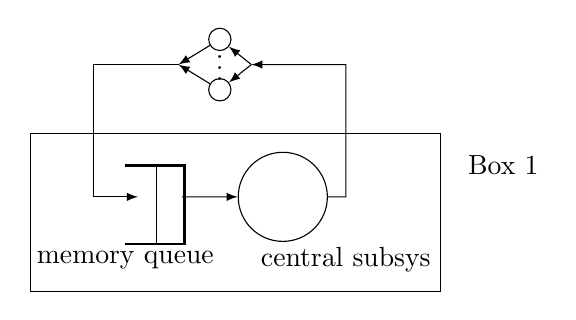
\begin{tikzpicture}[>=latex, scale=.8]
% the shapes
\node[draw, circle, inner sep=0.4cm] at (2.5,-0.5) (sys) {};
\path (0,0) pic {queue=1};
\node[draw, circle, inner sep = 0.1cm] at (1.5, 2) (u1) {};
\node[draw, circle, inner sep = 0.1cm] at (1.5, 1.2) (u2) {};
\node at ($(u1)!.4!(u2)$) {\vdots};
\node at (1, 1.6) (fakeleft){};
\node at (2, 1.6) (fakeright) {};

% the arrows
\draw[->] (u1) -- (fakeleft.west);
\draw[->] (u2) -- (fakeleft.west);
\draw[->] (fakeleft.west) -| (-.5,-.5) -- (0.2,-.5);
\draw[->] (.9,-.5) -- (sys.west);
\draw[->] (sys.east) -| (3.5,1.6) -- (fakeright.center);
\draw[->] (fakeright.center) -- (u1);
\draw[->] (fakeright.center) -- (u2);

%the names
\node at (0,-1.5) {memory queue};
\node at (3.5,-1.5) {central subsys};

%the box
\draw (-1.5,-2) rectangle (5,.5);
\node at (6,0) {Box 1};
\end{tikzpicture}

\begin{enumerate}
	\item $N_1 = X \cdot R$ (we can apply Little's law at box 1) \\
	$X = \frac{N}{R+Z} = \frac{100}{30} = 3.\overline{3}$\\
	$N_1 = 3.\overline{3} \cdot 10 = 33.\overline{3}$
	
	\item $R_{mq}=8'' \qquad N_{cs}=?$\\
	$N_{cs} = N_1 - N_{mq} = N_1 - X \cdot R_{mq} = 33.\overline{3} - 3.\overline{3} \cdot 8 = 33.\overline{3} - 26.\overline{6} = 6.\overline{6}$
\end{enumerate}
\end{frame}

\begin{frame}{Exercise 5 \cite{lazowska1984quantitative}}
 In a 30 minute observation interval, a particular disk was found to be
busy for 12 minutes. If it is known that jobs require 320 accesses to
that disk on average, and that the average service time per access is 25
milliseconds, what is the system throughput (in jobs/second)?
\end{frame}

\begin{frame}{Solutions}
$T=30'$ \ $B_d = 12'$ \ $V_d = 320$ \ $S_d = 25ms$ \ \ $X=?$

Two solutions:
\begin{enumerate}
	\item $X = \frac{U_d}{D_d} = \frac{\frac{B_d}{T}}{V_d \cdot S_d} = \frac{\frac{12'}{30'}}{320 \cdot 0.025 ''} = \frac{0.4}{8''} = 0.05 \frac{req}{sec}$ \vspace{.5cm}
	\item $X_d = \frac{U_d}{S_d}$ \\
	$X = \frac{X_d}{V_d} = \frac{\frac{U_d}{S_d}}{V_d} = \frac{U_d}{V_d \cdot S_d} = 0.05 \frac{req}{sec}$
\end{enumerate}
\end{frame}

\begin{frame}[allowframebreaks]{Exercise 6 \cite{lazowska1984quantitative}}
Consider the following measurement data for an interactive system
with a memory constraint:

\begin{tabular}{cc}
	T	&	1 hour	\\
	N	&	80	\\
	R	&	1 second	\\
	N in memory	&	6	\\
	C	&	36000	\\
	$U_{cpu}$	&	75\%	\\
	$U_{D1}$	&	50\%	\\
	$U_{D2}$	&	50\%	\\
	$U_{D3}$	&	25\%	\\
\end{tabular}
\break
\begin{enumerate}
	\item What was throughput (in requests / second)?
	\item What was the average ``think time''?
	\item On the average, how many users were attempting to obtain service
	(i.e., not ``thinking'')?
	\item On the average, how much time does a user spend waiting for
	memory (i.e., not ``thinking'' but not memory-resident) ?
\end{enumerate}
\end{frame}

\begin{frame}[allowframebreaks]{Solution}
$T = 1h$ \ $N=80users$ \ $R=1''$ \ $N' = 6$ \ $C=36000$\\
$U_{cpu} = .75$ \ $U_{d1} = .5$ \ $U_{d2} = .5$ \ $U_{d3} = .25$

\begin{enumerate}
	\item $X=?$ \ \ $X = \frac{C}{T} = \frac{36000 req}{1h} = \frac{36000 req}{3600''} = 10 \frac{req}{sec}$\\
	Notice that $\frac{N}{R}=\frac{80}{1} = 80 \frac{req}{sec} \neq X$ that's because in an interactive system we have thinking users and thus we cannot use Little's law.
	\item $Z=?$ \ \ $Z=\frac{N}{X}-R = \frac{80req}{10\frac{req}{sec}}-1''=7''$
	\item $N_{not\ think}=?$ \ \ $N''=X\cdot R=10\frac{req}{sec}\cdot 1 sec = 10 req$
	\item $?=R_{wait\ mem}=\frac{N_{wait\ mem}}{X} = \frac{N_{not\ think} - N_{in\ mem}}{X} = \frac{10-6}{10} = 0.4''$
\end{enumerate}

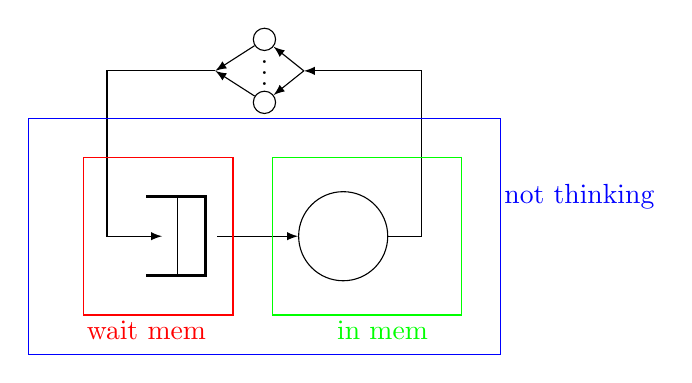
\begin{tikzpicture}[>=latex]
% the shapes
\node[draw, circle, inner sep=0.4cm] at (2.5,-0.5) (sys) {};
\path (0,0) pic {queue=1};
\node[draw, circle, inner sep = 0.1cm] at (1.5, 2) (u1) {};
\node[draw, circle, inner sep = 0.1cm] at (1.5, 1.2) (u2) {};
\node at ($(u1)!.4!(u2)$) {\vdots};
\node at (1, 1.6) (fakeleft){};
\node at (2, 1.6) (fakeright) {};

% the arrows
\draw[->] (u1) -- (fakeleft.west);
\draw[->] (u2) -- (fakeleft.west);
\draw[->] (fakeleft.west) -| (-.5,-.5) -- (0.2,-.5);
\draw[->] (.9,-.5) -- (sys.west);
\draw[->] (sys.east) -| (3.5,1.6) -- (fakeright.center);
\draw[->] (fakeright.center) -- (u1);
\draw[->] (fakeright.center) -- (u2);

%the box
\draw [blue] (-1.5,-2) rectangle (4.5,1);
\node [blue] at (5.5,0) {not thinking};

\draw [red] (-.8,-1.5) rectangle (1.1,.5);
\node [red] at (0,-1.7) {wait mem};

\draw [green] (1.6,-1.5) rectangle (4,.5);
\node [green] at (3,-1.7) {in mem};

\end{tikzpicture}
\end{frame}

\begin{frame}[allowframebreaks, fragile]{How to measure the service time?}
We know that $S_k = \frac{B_k}{C_k}$, but how can we measure it in a real situation?

We can build a simple monitoring infrastructure by using \url{https://prometheus.io/}, which collects metrics from monitored targets by scraping metrics HTTP endpoints on these targets.
It also offers a powerful query language.

\framebreak

Let's download prometheus and modify the \texttt{prometheus.yml} to scrape from localhost:
\begin{lstlisting}[basicstyle=\small]
# my global config
global:
  scrape_interval:     15s 

scrape_configs:
  - job_name: 'prometheus'
    static_configs:
    - targets: ['localhost:9090']

  - job_name: 'example_python'
    static_configs:
    - targets: ['localhost:9999']
\end{lstlisting}

\framebreak

And write a simple python example:
\begin{lstlisting}[basicstyle=\tiny]
import time
import numpy as np
from prometheus_client import start_http_server, Counter

def server():
    sleep = np.random.normal(2)
    sleep = int(max(0, sleep))
    time.sleep(sleep)

if __name__ == '__main__':
    completions = Counter('completions', 'number of completed requests')
    time_passed = Counter('time_passed', 'amount of time passed')
    start_http_server(9999)
    
    for n in range(60):
        tic = time.time()
        server()
        toc = time.time()
        time_passed.inc(toc-tic)
        completions.inc(1)
\end{lstlisting}

\framebreak

Which value do we expect for the service time?

Now start prometheus, run the script and head to \url{http://localhost:9090}.
With the tab \emph{graph} we can check the metrics \emph{completions\_total} and \emph{time\_passed\_total},
we can also graph the value of \emph{time\_passed\_total /  completions\_total}, obtaining an estimate of the service time of our server.

\end{frame}

\begin{frame}{References}
\printbibliography
\end{frame}

\end{document}
